\documentclass{beamer}
\usetheme{Warsaw}
\usepackage{nhtvslides}
\usepackage{graphicx}
\usepackage{amssymb}
\usepackage{pifont}
\usepackage{listings}
\lstset{language=CAML,
basicstyle=\ttfamily\footnotesize,
frame=shadowbox,
breaklines=true}
\usepackage[utf8]{inputenc}

\newcommand{\cmark}{\ding{51}}%
\newcommand{\xmark}{\ding{55}}%

\title{Detecting dyslexia}
\subtitle{Building a game for dyslexia detection in young children}

\author{Dr. Giuseppe Maggiore \and Dr. Marie Postma}

\institute{NHTV University of Applied Sciences \\ 
Breda, Netherlands}

\date{}

\begin{document}
\maketitle

\begin{frame}{Agenda}
\tableofcontents
\end{frame}

\section{Detecting dyslexia}
\begin{slide}{Detecting dyslexia}{Sound and dyslexia}{
\item Children between 8 and 11 years old \cite{LOCAL_GLOBAL_DYSLEXIA}
\item Ability to parse sound correlated with dyslexia
}\end{slide}

\begin{slide}{Detecting dyslexia}{Sound and dyslexia}{
\item Processing of local/global pitch in 4-tone sequences
\item Local, but not global issues in dyslectic children
\item Processing of local/global pitch done by different brain parts
\item Left hemisphere processes local, right global
\item Left hemisphere deficits correlated with dyslexia
}\end{slide}

\begin{frame}{Sound and dyslexia}
\center
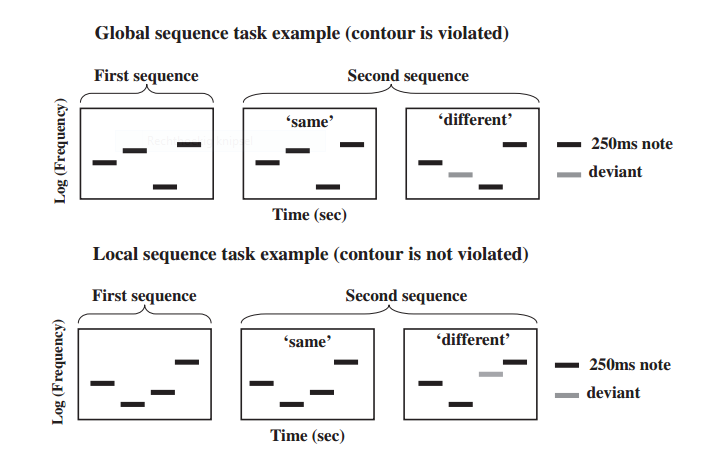
\includegraphics[height=5cm]{Pics/local_global.png}
\end{frame}

\begin{slide}{Detecting dyslexia}{Test}{
\item Experiment 1: 40 pairs of 4-tone sequences (20 same, 20 different)
\item Experiment 2: 30 trials of 2-tone sequences (15 rising and 15 falling)
}\end{slide}

\begin{textslide}{Detecting dyslexia}{Problem}{
\textbf{Attention/interest span of young children} (ePrime)
}\end{textslide}

\begin{slide}{Detecting dyslexia}{Test issues}{
\item Limits applicability of test
\item How about even younger children?
\item How about longer/combined tests?
}\end{slide}

\begin{textslide}{Detecting dyslexia}{Our goal}{
\textbf{Increase interest of children on the tests} to improve focus/duration 
}\end{textslide}


\section{Serious games}
\begin{slide}{Serious games}{Serious games}{
\item Let us shift our attention away from dyslexia...
\item ...and let us focus on video games instead
\pause
\item Video games are powerful tools for:
\begin{itemize}
\item Entertainment
\item User immersion
\item Communication
\item Training (both within and without entertaining games)
\end{itemize}
}\end{slide}

\begin{frame}{Training in entertainment games}
\center
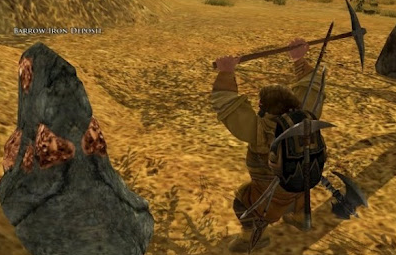
\includegraphics[height=5cm]{Pics/grinding.png}
\end{frame}

\begin{slide}{Serious games}{Games for training}{
\item As a supporting tool for training \cite{GAMES_FOR_TRAINING}
\begin{itemize}
\item \textit{military}
\item \textit{crane operation}
\item \textit{medicine}
\item ...
\end{itemize}
}\end{slide}

\begin{frame}{Serious games}
\center
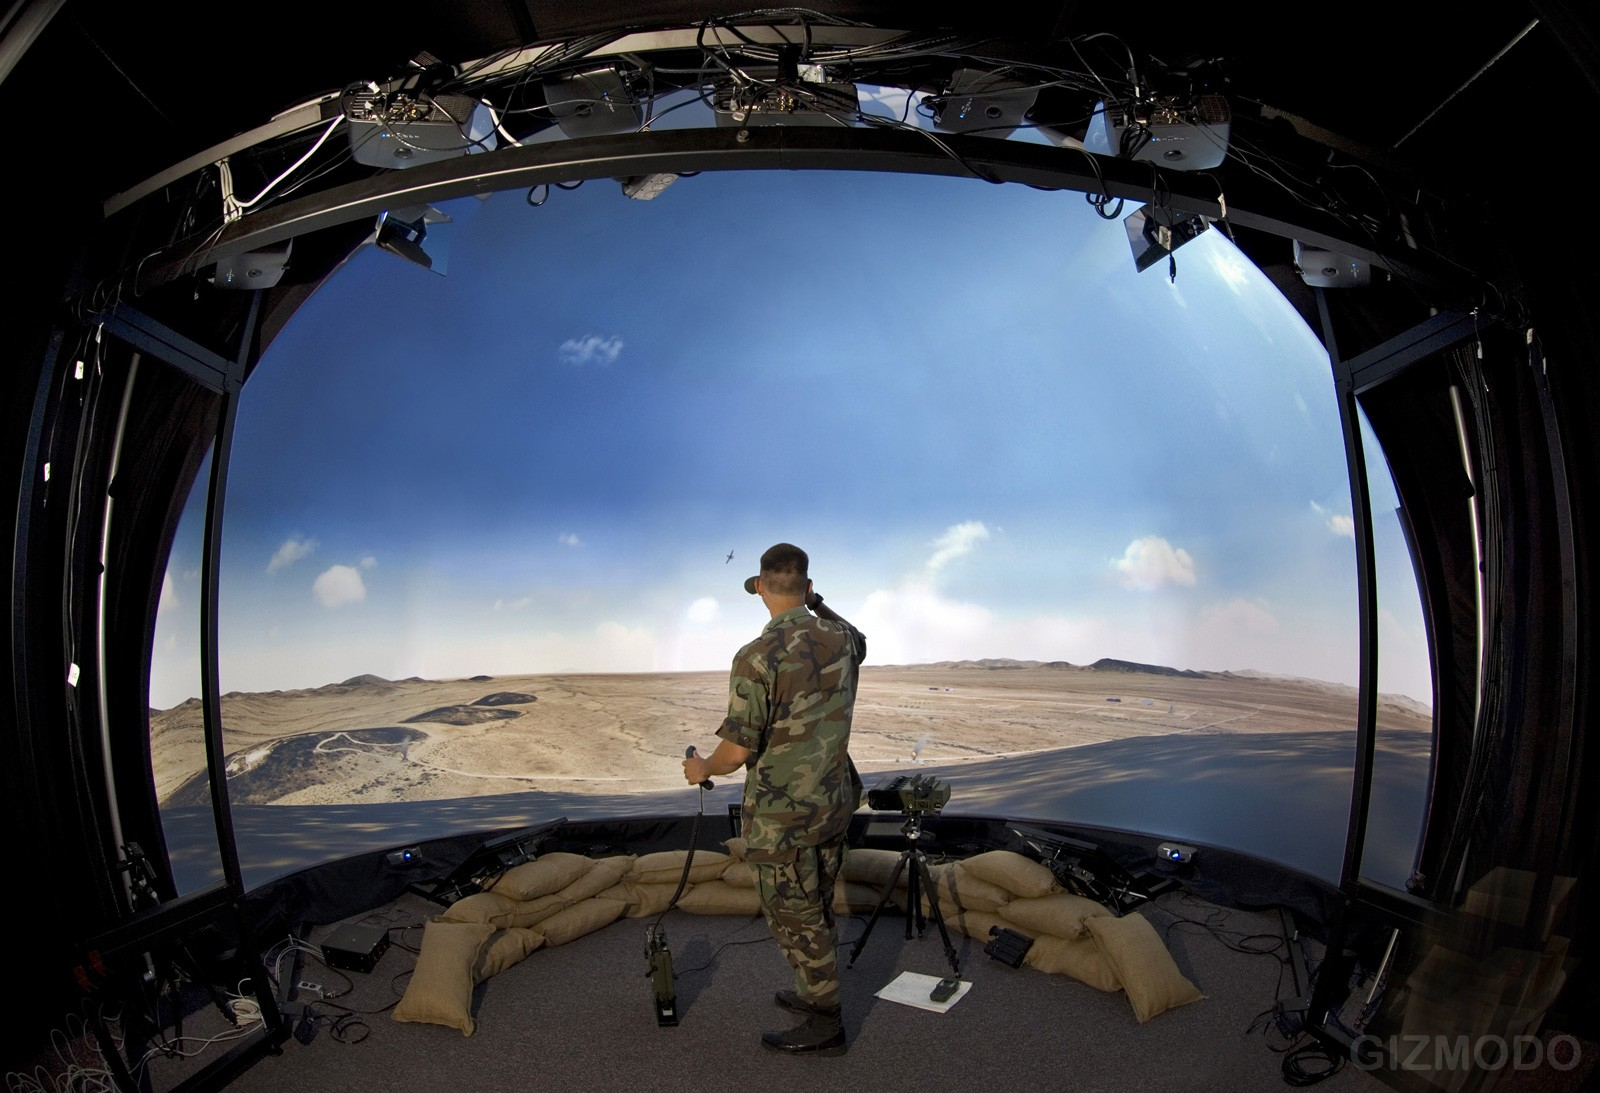
\includegraphics[height=5cm]{Pics/military_simulator.png}
\end{frame}

\begin{frame}{Serious games}
\center
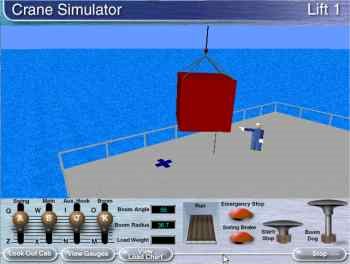
\includegraphics[height=5cm]{Pics/crane_simulator.png}
\end{frame}

\begin{frame}{Serious games}
\center
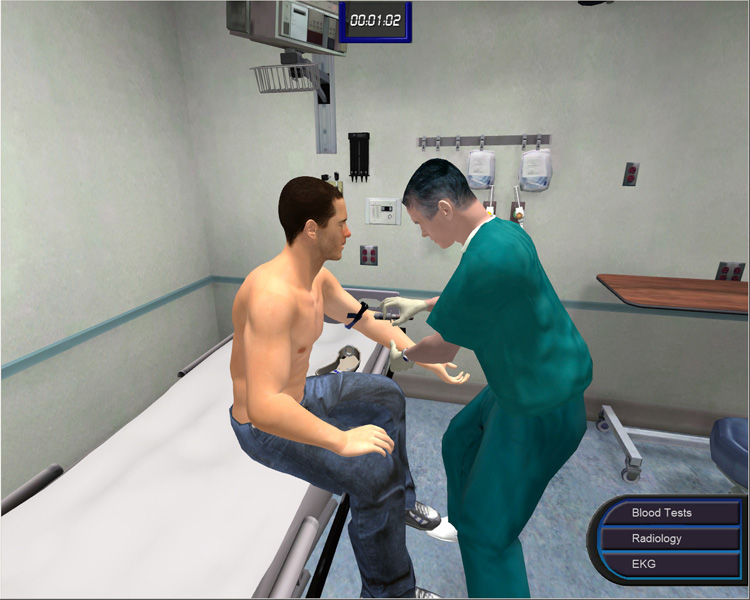
\includegraphics[height=5cm]{Pics/medical_simulator.png}
\end{frame}

\begin{slide}{Serious games}{Games for education}{
\item As a supporting tool for education \cite{GAMES_FOR_EDUCATION}
\begin{itemize}
\item Math
\item Chemistry
\item History
\item ...
\end{itemize}
}\end{slide}

\begin{frame}{Serious games}
\center
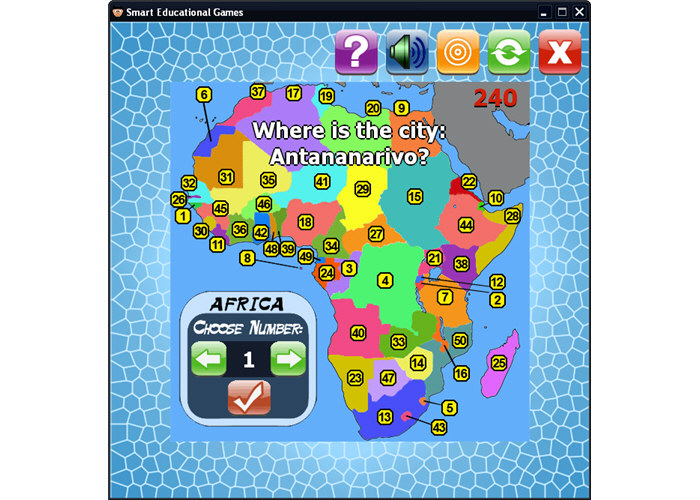
\includegraphics[height=5cm]{Pics/game_for_education.png}
\end{frame}

\begin{frame}{Serious games}
\center
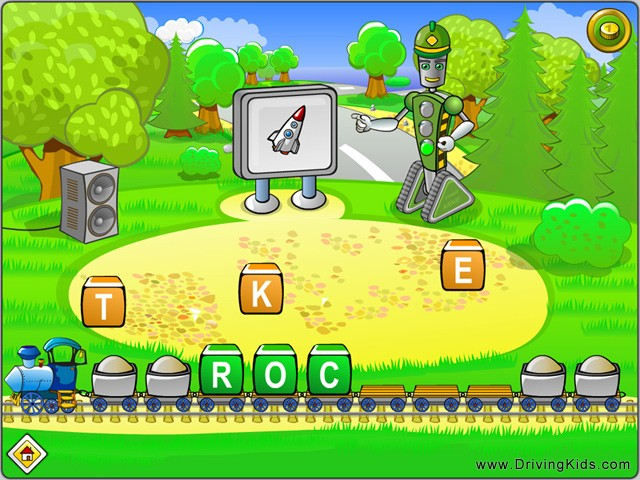
\includegraphics[height=5cm]{Pics/game_for_education_2.png}
\end{frame}

\begin{textslide}{Serious games}{The power of games?}{
\textbf{What makes games so powerful?}
}\end{textslide}

\begin{slide}{Serious games}{Power of games}{
\item A large field of literature on the topic
\begin{itemize}
\item Visual gratification
\item Visual metaphor
\item Sense of reward and progression
\end{itemize}
}\end{slide}

\begin{slide}{Serious games}{Visual gratification}{
\item Colours
\item Shapes
\item Visual coherence
}\end{slide}

\begin{frame}{Serious games}
\center
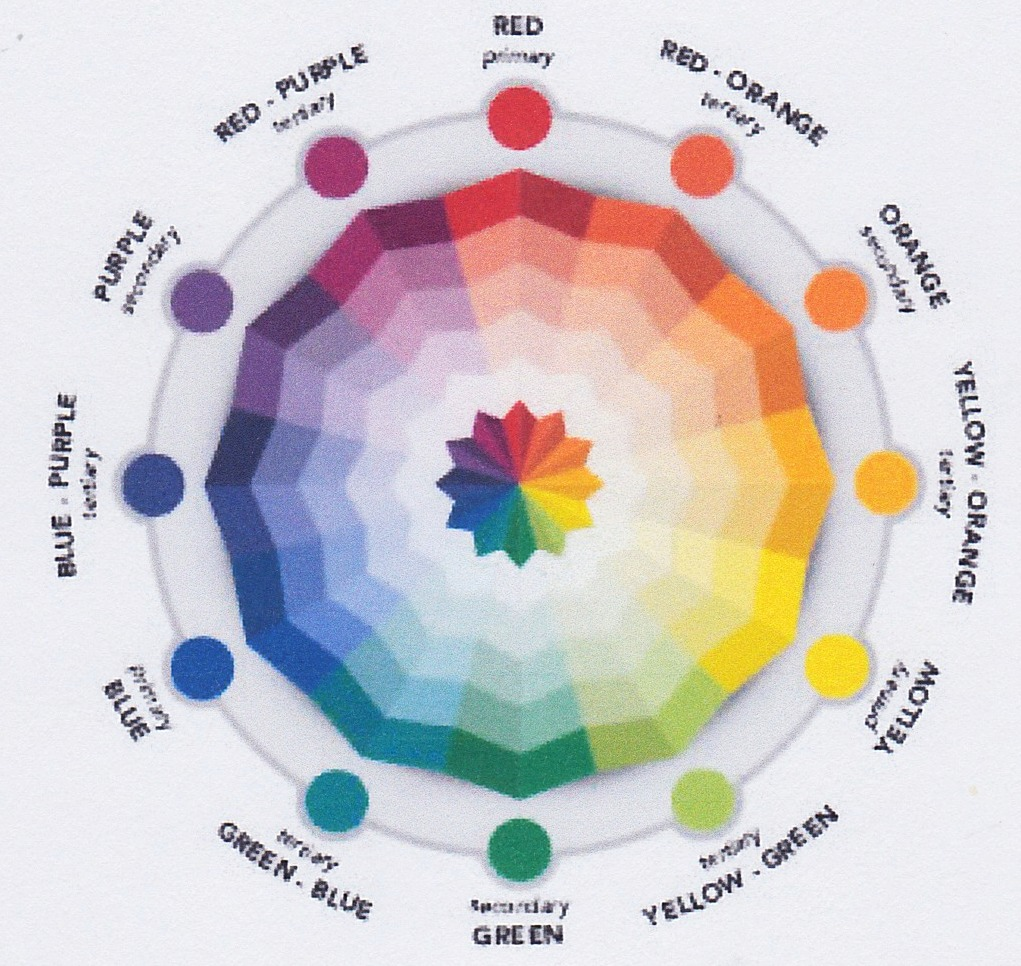
\includegraphics[height=5cm]{Pics/color_combinations.png}
\end{frame}

\begin{slide}{Serious games}{Visual metaphor}{
\item Recognizable items
\item Recognizable scenes
\item Recognizable actions
}\end{slide}

\begin{frame}{Serious games}
\center
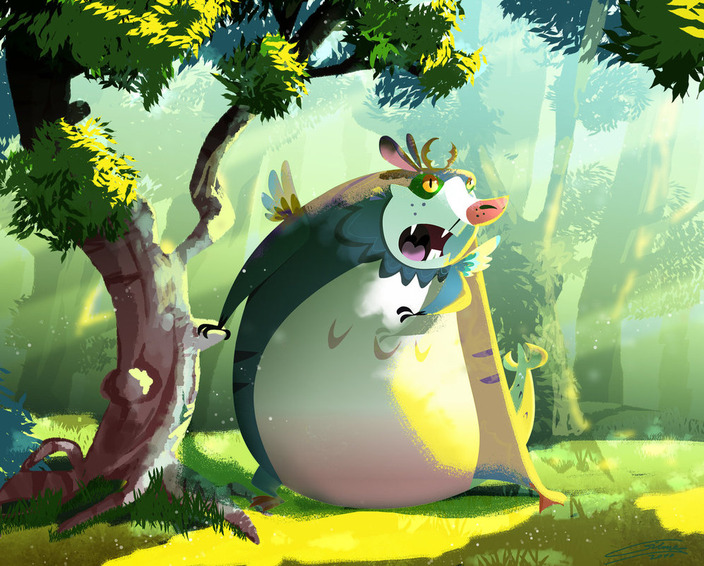
\includegraphics[height=5cm]{Pics/woods_metaphor.png}
\end{frame}

\begin{slide}{Serious games}{Sense of reward and progression}{
\item Actions have some (meaningful) effect on the world
}\end{slide}

\begin{frame}{Serious games}
\center
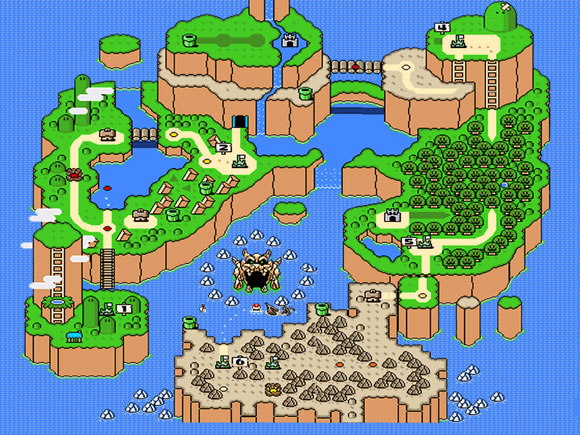
\includegraphics[height=5cm]{Pics/mario_world.png}
\end{frame}

\begin{frame}{Serious games}
\center
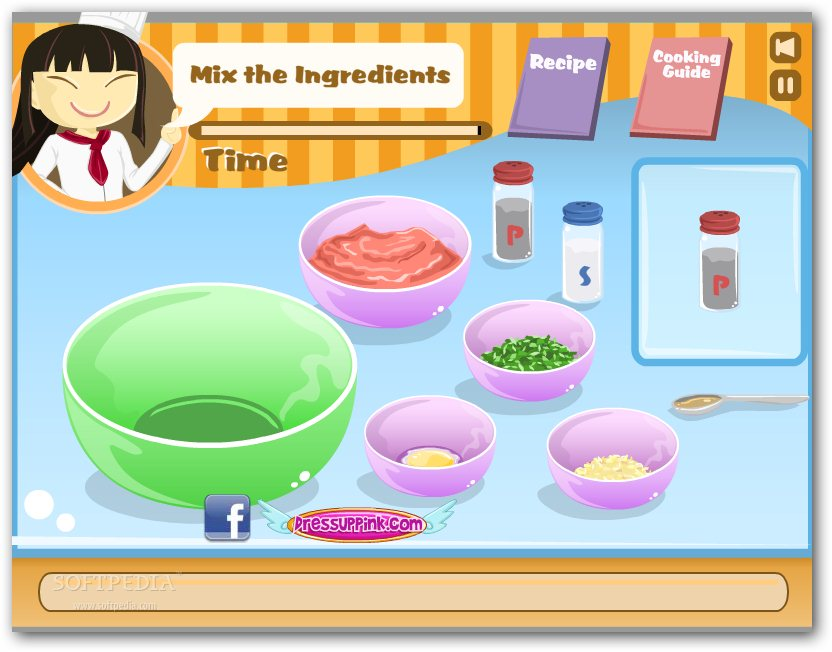
\includegraphics[height=5cm]{Pics/cooking_game.png}
\end{frame}

\begin{textslide}{Serious games}{Our goal}{
\textbf{Build a game for testing dyslexia in children}
}\end{textslide}

\section{A game for dyslexia detection}
\begin{slide}{A game for dyslexia detection}{Hazards}{
\item \textbf{Do not influence the outcome}
\begin{itemize}
\item Avoid rewards for success (``feel bad for being dyslectic?'')
\item Avoid implicit bias towards some options and solutions
\end{itemize}
}\end{slide}

\begin{slide}{A game for dyslexia detection}{Core idea}{
\item Fable-like theme
\item A ``generically magical'' stroll in the woods
}\end{slide}

\begin{slide}{A game for dyslexia detection}{Core idea}{
\item Anthropomorphic fox with a trumpet
}\end{slide}

\begin{frame}{A game for dyslexia detection}
\center

\includegraphics[width=10cm]{Pics/fox.png}
\end{frame}

\begin{slide}{A game for dyslexia detection}{Core idea}{
\item Birds try to imitate the sounds
}\end{slide}

\begin{frame}{A game for dyslexia detection}
\center

\includegraphics[width=10cm]{Pics/bird.png}
\end{frame}

\begin{slide}{A game for dyslexia detection}{Core idea}{
\item Determine if the bird imitated the sound correctly or not
}\end{slide}

\begin{frame}{A game for dyslexia detection}
\center

\includegraphics[height=5cm]{Pics/yes_no_button.png}
\end{frame}

\begin{slide}{A game for dyslexia detection}{Core idea}{
\item A stroll in the woods (sense of progression)
}\end{slide}

\begin{frame}{A game for dyslexia detection}
\center
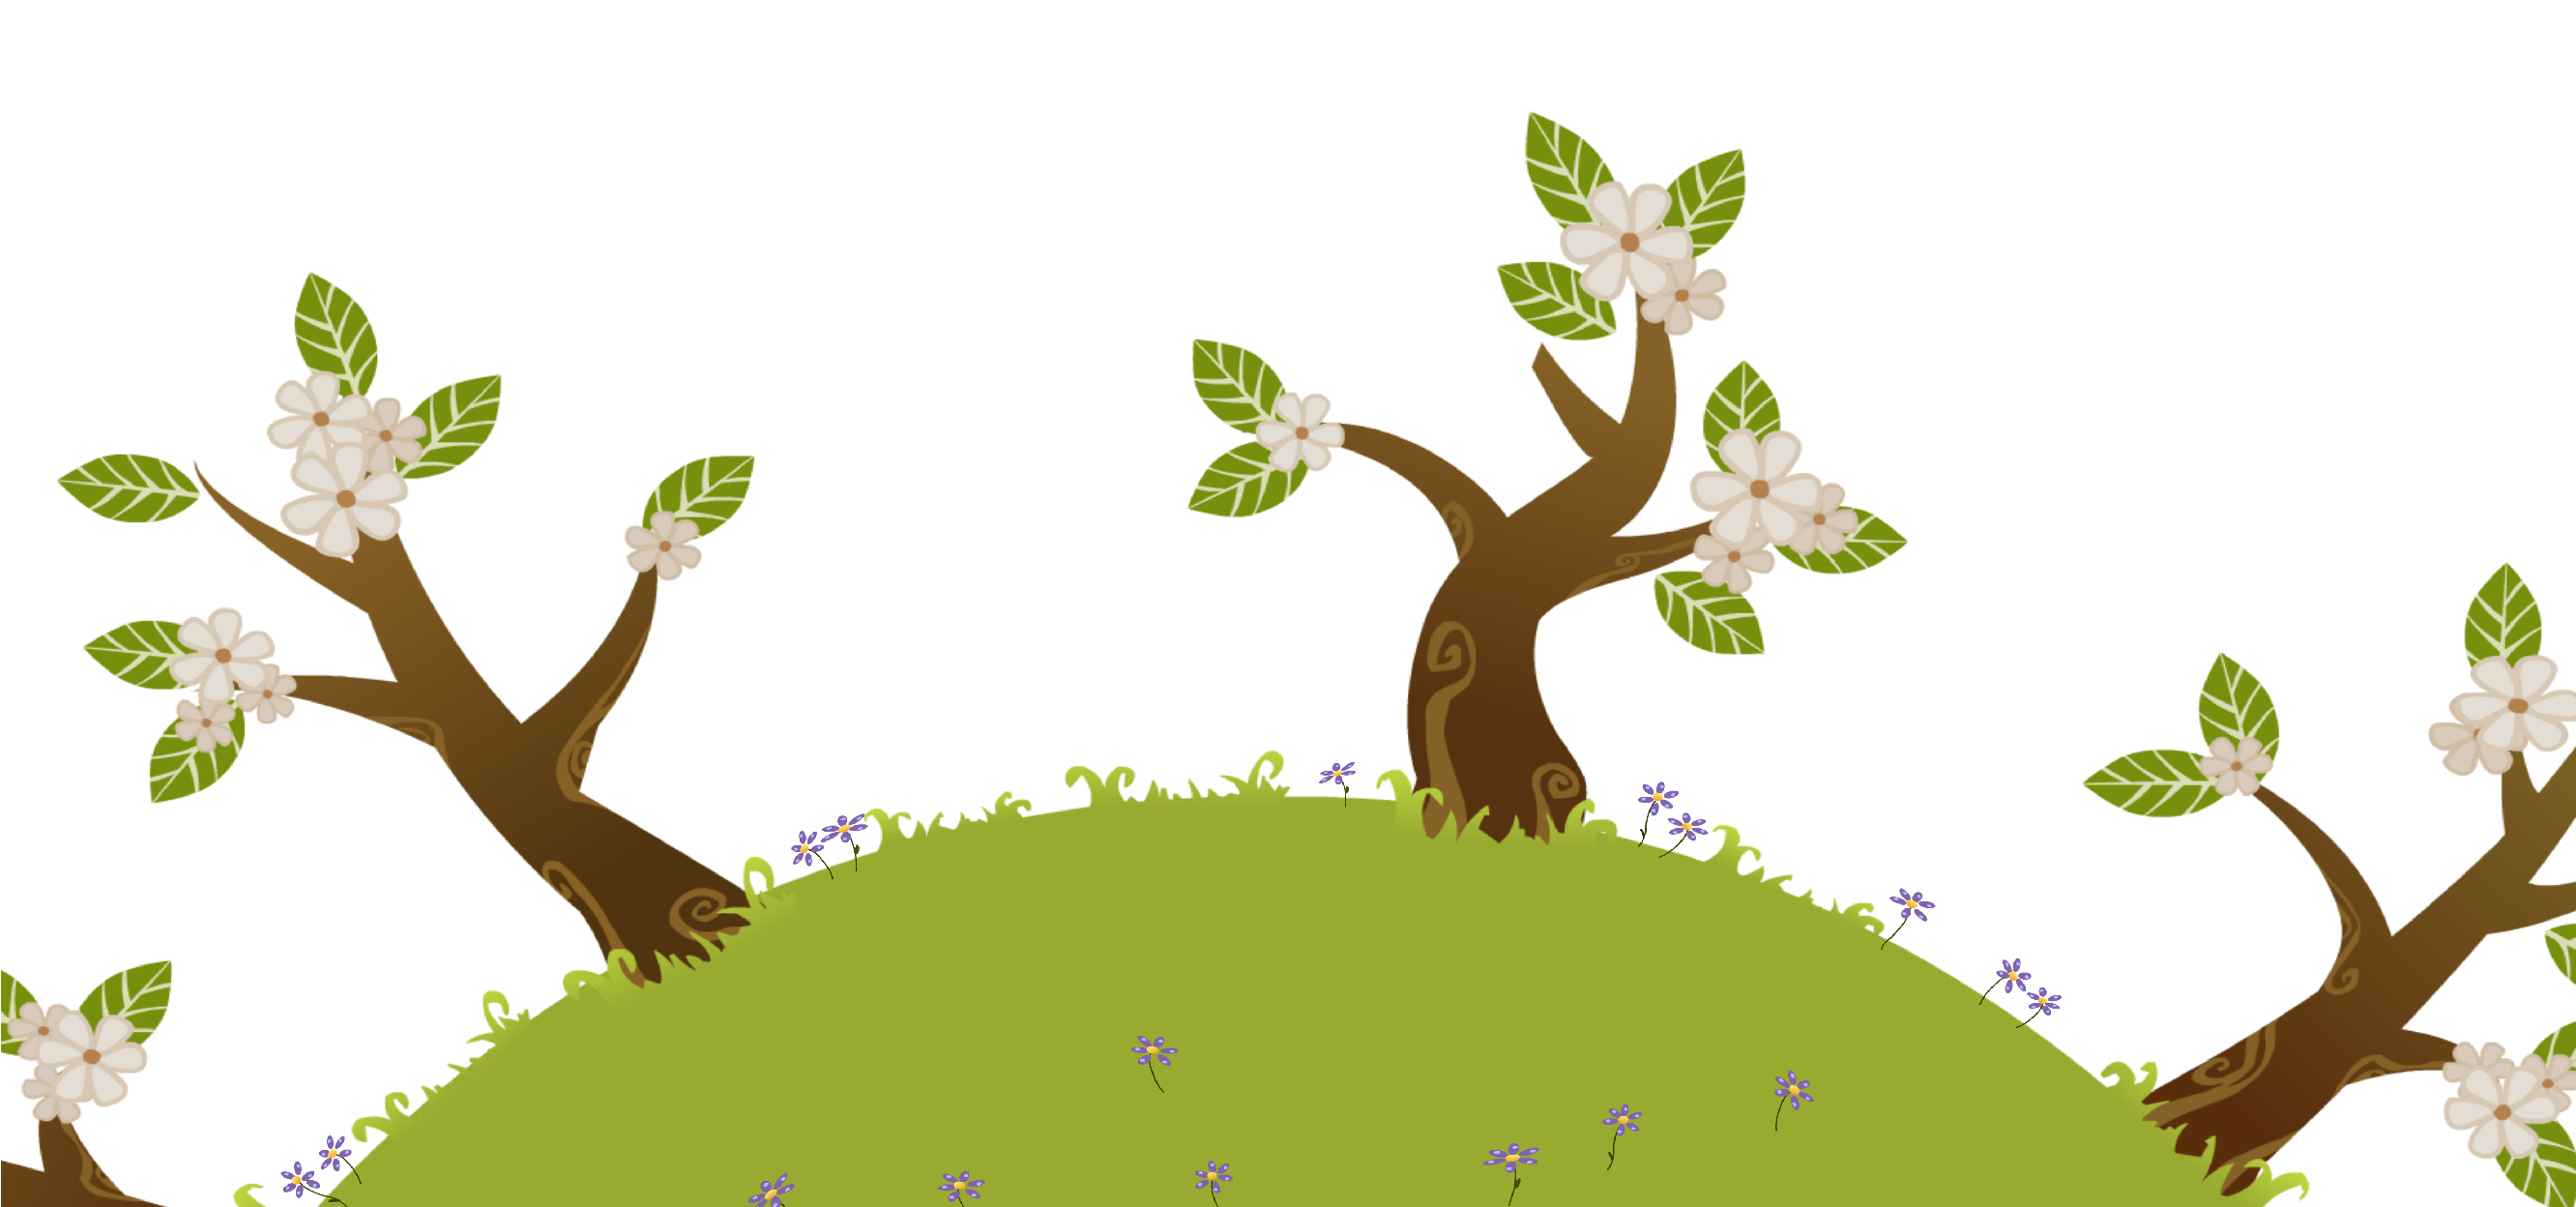
\includegraphics[height=5cm]{Pics/woods.png}
\end{frame}

\begin{slide}{A game for dyslexia detection}{Core idea}{
\item Example tasks for initial tutorial session
\item Non-verbal, very quick
\item Use simple animations
}\end{slide}

\begin{frame}{A game for dyslexia detection}
\center
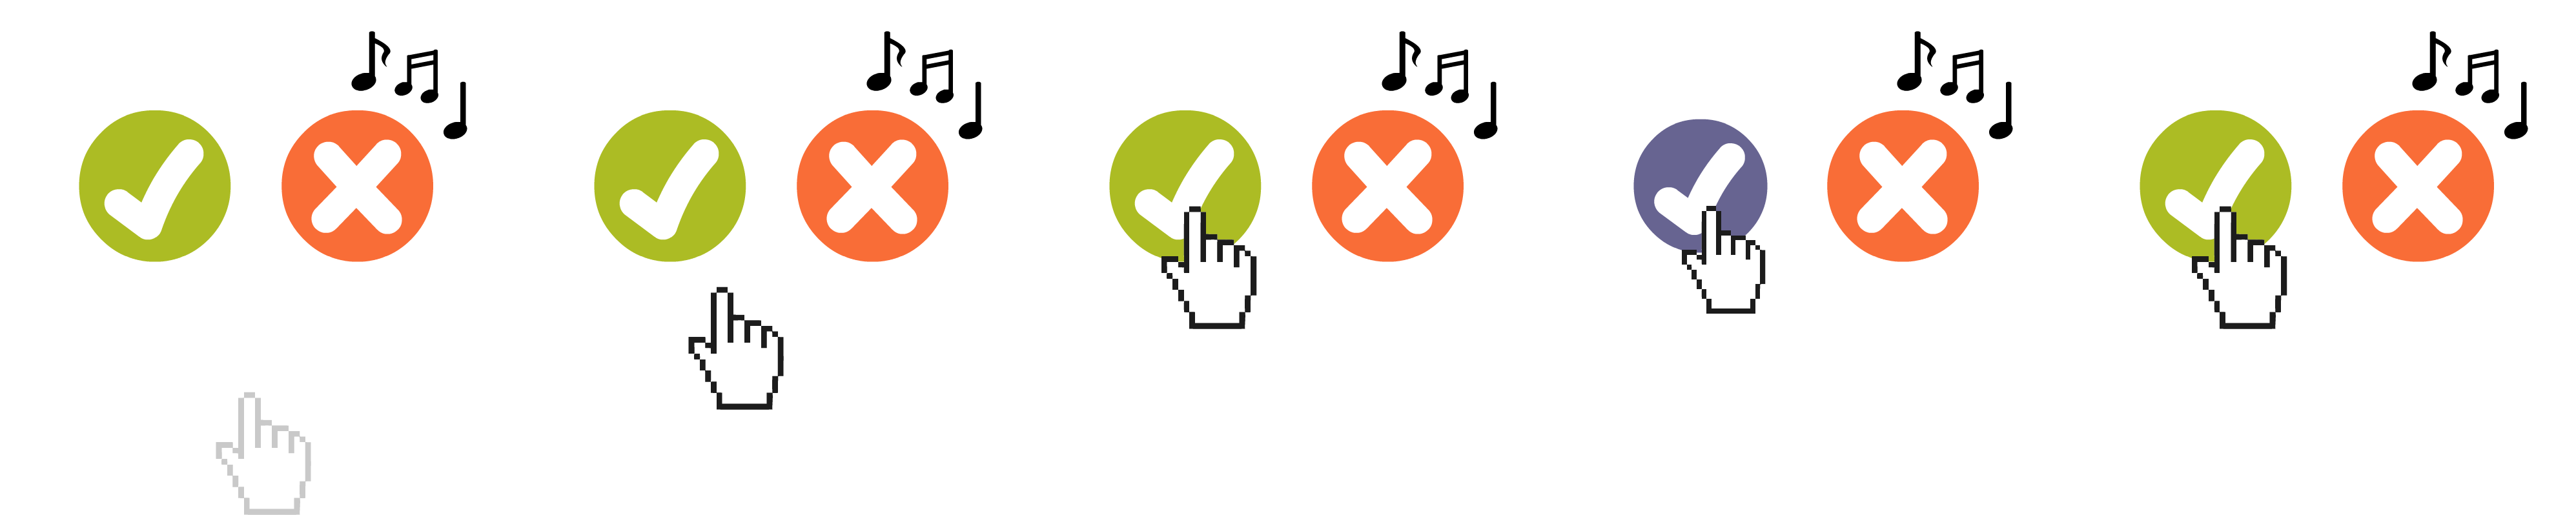
\includegraphics[width=10cm]{Pics/animated_buttons.png}
\end{frame}

\begin{slide}{A game for dyslexia detection}{Additional items}{
\item Touch input for immediacy
\pause
\item Gathering data for analysis
\pause
\item Customizable experiments
}\end{slide}

\begin{textslide}{A game for dyslexia detection}{Demo}{
\textbf{Let's see it in action}
\center
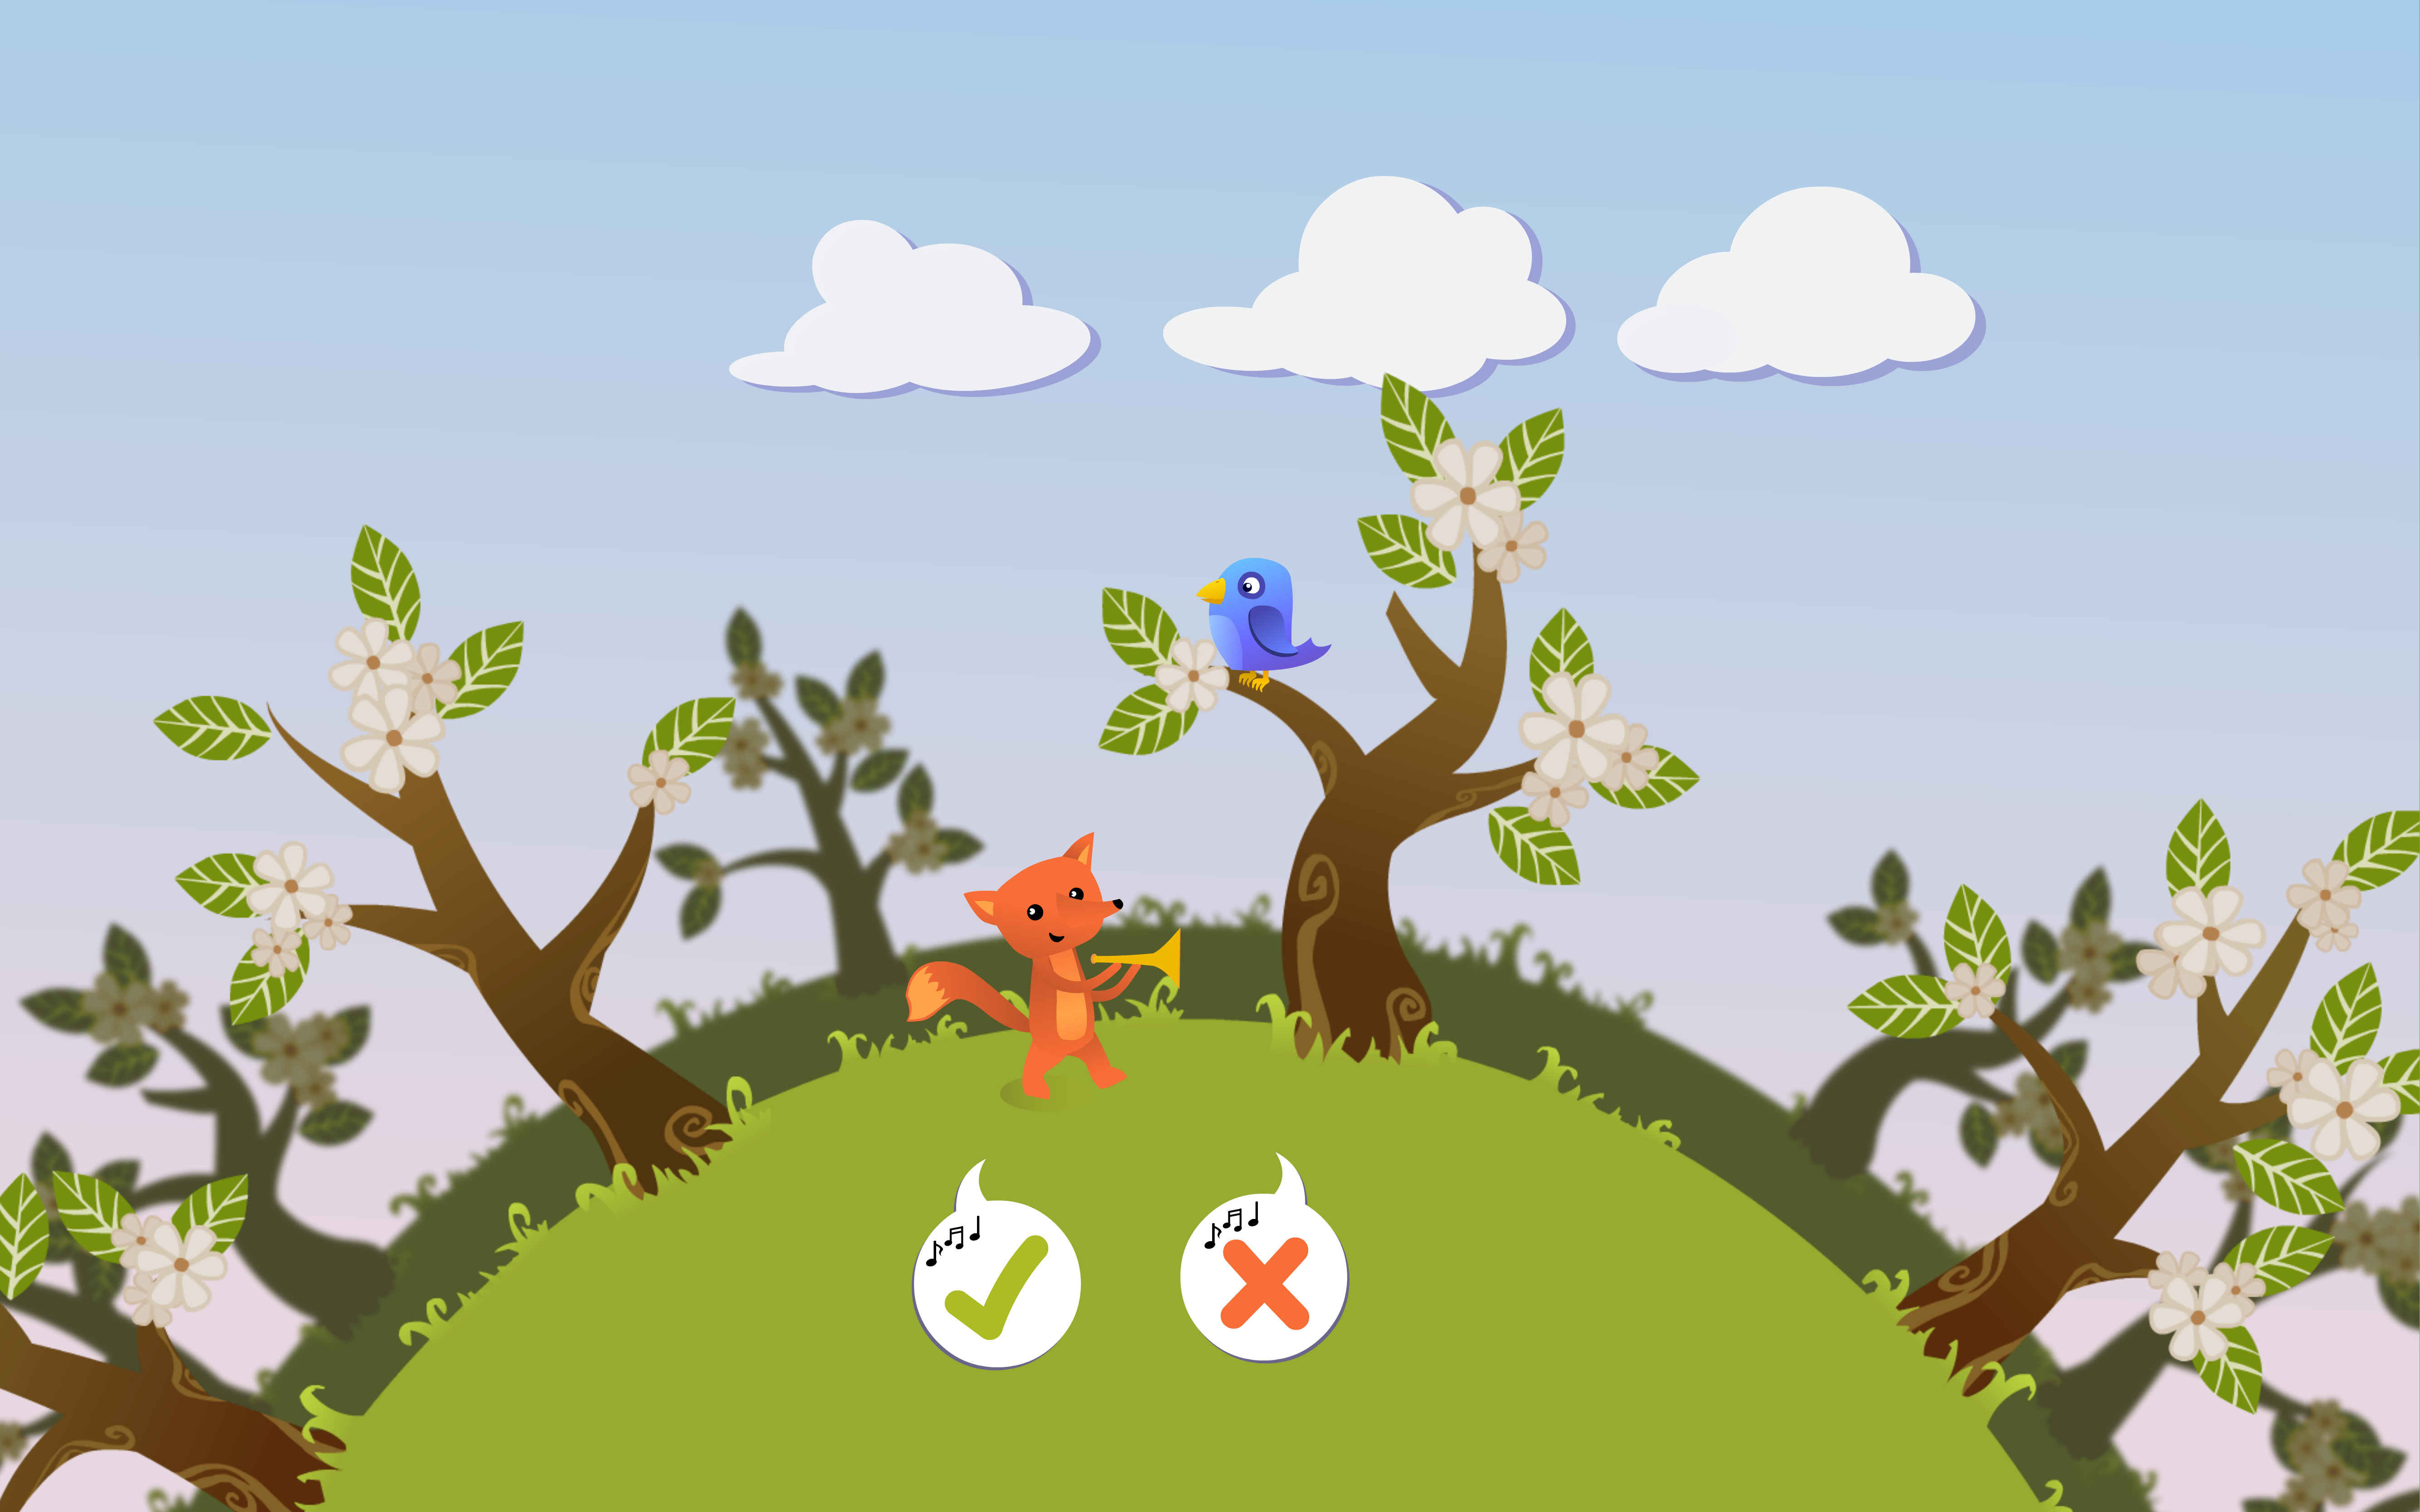
\includegraphics[height=5cm]{Pics/full_view.png}
}\end{textslide}

\section{About the development process}
\begin{slide}{Game technologies}{Standard technologies}{
\item Support for typical game structures
\item Very powerful at capturing typical solutions to graphics, sound, input, and physics issues in games
\pause
\item Unfortunately, they do not really apply to research games
}\end{slide}

\begin{slide}{Game technologies}{Research games}{
\item Atypical mechanics
\item Unclear requirements
\begin{itemize}
\item It is still a research process
\item Researchers expert in their field, not games (opposite applies to us)
\item Even if they sign, they cannot envision product from specifications
\item Even if we make a proposal, we do not fully understand the research
\end{itemize}
}\end{slide}

\begin{slide}{Game technologies}{Research games}{
\item We have built Casanova, a programming language for extremely fast prototyping of games \cite{CASANOVA}
\item A different way of engineering games
\item When compared with existing engines like Unity 3D, it does not excel in:
\begin{itemize}
\item Performance
\item Physics
\item Graphics
\end{itemize}
\item What it excels in, is development time and flexibility
\begin{itemize}
\item Lots of iteration
\item Strange/unusual requirements
\end{itemize}
}\end{slide}

\begin{slide}{Game technologies}{Research games}{
\item \textbf{Three whole prototypes}, two entirely thrown away
\item Capture the mechanics \textit{by showing them to the researcher}
\item Iterative refinement of the requirements
\item Art created and integrated only last
\item Final price tag was ridiculously low
\item Very positive final feedback on \textit{product and process}
}\end{slide}

\begin{slide}{Conclusions}{Serious games for testing and children}{
\item Testing conditions such as dyslexia is hard...
\item ...especially when the subject is an impatient child
\item Turn the test into something fun and living through games
\item Make such a test really cheap and accessible (home, at school, etc.)
}\end{slide}

\begin{slide}{Conclusions}{Serious games for testing and children}{
\item Building research games does not match well with existing technologies
\item Unusual requirements, intrinsic communication issues with researcher
\item We have built our own technology centred around this process
\item Make building such games really cheap and accessible
}\end{slide}

\begin{frame}{That's it}
\center
\fontsize{18pt}{7.2}\selectfont
Thank you!
\end{frame}

\begin{frame}{That's it}
\center
\fontsize{18pt}{7.2}\selectfont
With heartfelt thanks to Aske and Pieter for all their support so far.
\end{frame}

\begin{frame}[allowframebreaks]
\frametitle{References}
\bibliographystyle{plain}
\bibliography{bibliography}
\end{frame}

\end{document}
